% ASTR400B directed research. Assingment 2

\documentclass[twocolumn, trackchanges]{aastex7}
\usepackage{graphicx}
\usepackage{wrapfig}   

\begin{document}

\title{MW-M31 Major Galaxy Merger Remanent Rotation Profile}

\author{Hina Suzuki}
\altaffiliation{Steward Observatory and Department of Astronomy}
\altaffiliation{Department of Electrical and Computer Engineering}
\affiliation{University of Arizona}
\email[show]{hinas@arizona.edu}  

\section{Introduction} 
%cite 3 papers

% Par1: Define your proposed topic and how it pertains to Galaxy Evolution.
Galaxy mergers are one of the most significant processed shaping the structure, kinematics, and morphology of galaxies. When two galaxies of comparable mass merge, their stellar and dark matter components undergo significant dynamical transformations, leading to change in rotation, redistribution of angular momentum. Understanding these processed provides insight into how galaxies evoles and form structures we observe today. In this study, I focus on stellar disk and bulge kinematics after a major merger, examining the Milky Way (MW) and Andromeda (M31) system using numerical simulation. The goal is to study how angular momentum is redistributed and whether the remnant behaves as fast or slow rotator. 

% Par2: State why this topic matters to our understanding of galaxy evolution.
The kinematics of major mergers remnants provide crucial insight into the structural transformation of galaxies. Angular momentum redistribution determines whether a remnant is rotationally supported, or dispersion-dominated. Additionally, rotation curves in post-merger system helps constrain the dark matter distribution, offering a deeper understanding of galaxy dynamics. Understanding this process is connect present-day galaxy profiles to their merger history. By studying MW/M31 merger, we can model galaxy merger precisely given detailed observational data, and better understand how kinematic structure of galaxies evolve over time. 

% Par3: Overview our current understanding of the topic in galaxy evolution, broadly.
Advancements in high-resolution simulations, deep-space observations, and theoretical models have significantly improved our understanding of galaxy evolution. Observations from JWST have provided insights into the earliest galaxies. Large-scale surveys, such as SDSS and HST studies, have helped identify classification of galaxy structure. On the theoretical side, large-scale simulations such as EAGLE \citep{2015MNRAS.446..521S} have improved our ability to model galaxy mergers, gas accretion, and structural transformations. Recent studies explored merger remnants formed by various theoretical galaxies, suggesting that gas-rich major mergers tend to produce fast-rotating remnants, whereas slow-rotating remnants typically require multiple mergers \citep{Cox_2006, Naab}. Also, rotation curve showed that angular momentum was carried by old stars in the case of dissipational mergers.

\begin{figure}
  \centering
  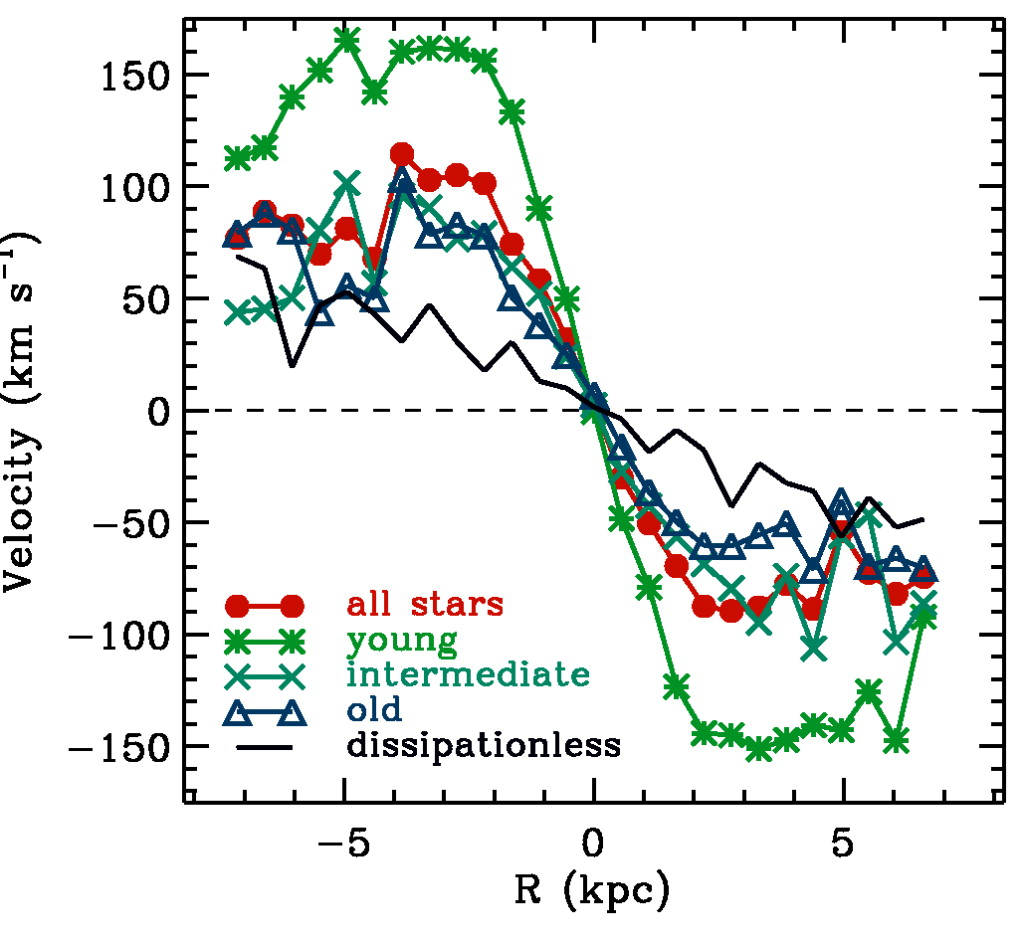
\includegraphics[width=\columnwidth]{RA2/rotationref.jpg}
  \caption{The rotation curve about rotational axis of the dissipational galaxy major merger remnants, segmented by particle types. \citep{Cox_2006}}
  \label{fig:rotationref}
\end{figure}
However, because MW and M31 are only moderately gas-rich and only partially dissipational, there are insufficient predictions regarding the rotational properties of their merger remnant. This raises an open question: Will the MW/M31 remnant retain significant rotation, or will it resemble a slow rotator typically found in massive elliptical? Despite these advancements, challenges remain in interpreting observational data and integrating theoretical models, particularly regarding rotation profiles in merger remnants. The MW/M31 system presents an excellent case study to refine our understanding of how major mergers affect galaxy kinematics. By combining observational constraints with detailed numerical simulations, we can develop more precise models of galaxy evolution and rotational transformation.

% Par4:
This raises an open question: Will the MW/M31 remnant retain significant rotation, or will it resemble a slow rotator typically found in massive elliptical? Despite these advancements, challenges remain in interpreting observational data and integrating theoretical models, particularly regarding rotation profiles in merger remnants. The MW/M31 system presents an excellent case study to refine our understanding of how major mergers affect galaxy kinematics. By combining observational constraints with detailed numerical simulations such as those collision less  N-body simulation \citep{van_der_Marel_2012}, we can develop more precise models of galaxy evolution and rotational transformation.

\section{Proposal} 
\subsection{Topic} 
% Subsec1: This Proposal. What specific question(s) will you be addressing using the simulation? You only need to pick one - think about how much time you have realistically!
My project aims to understand wether MW/M31 merger remnant is fast rotator or slow rotator, examining velocity distribution, velocity dispersion, and velocity profile $\frac{V}{\sigma}$.

\subsection{Method}
% One figure/ diagram
% How will you approach the specific question using the simulation data? Define all relevant equations and terms. Here you should outline the codes you’d need to write - each question will need a unique code solution. This can be described in general terms, but all steps need to be outlined (including what particle types/properties will you select and how you will select them, and specify which snapshots will you use).
This work combines individual N-body simulations of MW and M31 galaxy into one system, as a remanent. We will analyze the kinematics of the remnant by studying its velocity dispersion and rotation curve by using low resolution simulation at 8.0Gyrs from now, because this is the time where two galaxies merged and relative velocity converged sufficiently. Here listed are tasks to be done for this project. 
\begin{itemize}
    \item Obtain low resolution simulation data, snapshot number 560 into dataset.    
    \item  Develop script to combine disk and bulge particles from both Milky Way and M31 into single dataset after galaxies have merged. 
    \item Recalculate center of mass of the system, followed by relative position of particles from the center of mass. 
    \item Calculate angular momentum vector to adjust coordinate system so that rotation axis is cartesian z axis. 
    \item Make plot of rotation curve, to determine maximum rotation about major axis.
    \item Calculate velocity dispersion of merger remanent, using particles within effective radius. 
    \item Implement a script to determine statistical velocity dispersion of merged structure, using following equations.
        \begin{equation}
            \sigma ^2 = \frac{1}{N} \sum_{i=1}^{N} (v- \langle v \rangle)^2 
        \end{equation}
        
        \begin{equation}
            \langle v \rangle = \frac{1}{N}  \sum_{j=1}^{N} v_j
        \end{equation}
    , where $\sigma $ is the variance, $\langle v \rangle $ is mean velocity, N is number of particles in simulation, and $v$ is velocity of each particle. We will implement those using NumPy functions: numpy.mean(), numpy.std().
    \item Construct plots of radial profile of the rotation velocity, radial profile of the velocity dispersion, and the radial profile of the rotation to dispersion ratio for the merger remnant, as we did in Lab7, using CenterOfMass function in the simulation with particles in remanent.
\begin{figure}[h]
  \centering
  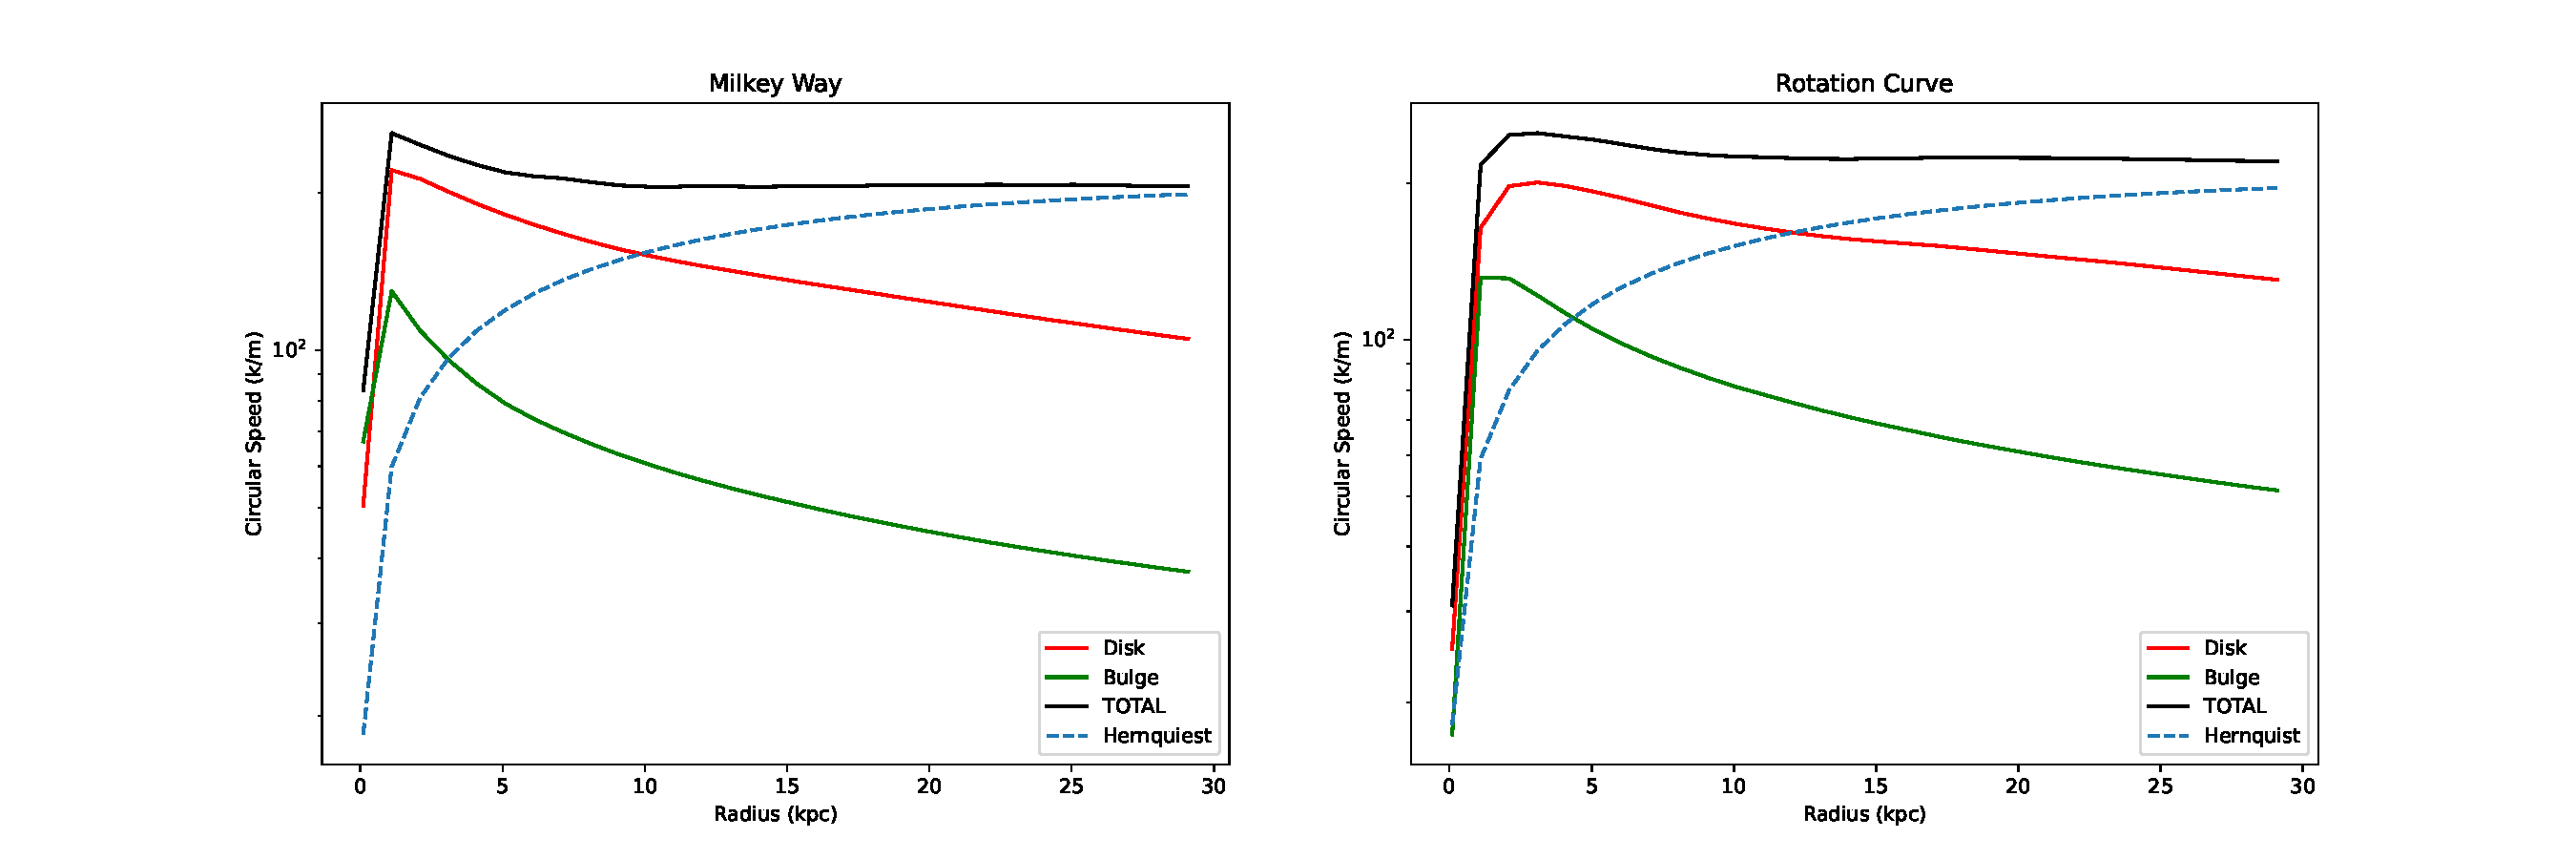
\includegraphics[width=\columnwidth]{RA2/Rotation.pdf}
  \caption{Example of rotation curves. Left panel is Milky Way Galaxy at present day, and Right panel is Andromeda Galaxy. Color code: Red-Disk, Green-Bulge, Black-Disk and Bulge}
  \label{fig:lab7example}
\end{figure}

\end{itemize}

\subsection{Hypothesis} 
% What is your hypothesis for what you will find? Why do you think this will occur?
My hypothesis is that the MW/M31 major merger remnant will retain some degree of rotation but will not qualify as a fast rotator, as neither galaxy is particularly gas-rich. The remnant is expected to behave a slower rotation compared to the pre-merger galaxies, as the system is likely to inherit some of its initial kinematic properties while undergoing angular momentum redistribution during the merger process.

\bibliography{refs}
\bibliographystyle{aasjournal}


\end{document}

